% Options for packages loaded elsewhere
\PassOptionsToPackage{unicode}{hyperref}
\PassOptionsToPackage{hyphens}{url}
%
\documentclass[
  english,
  man,man,floatsintext]{apa6}
\usepackage{amsmath,amssymb}
\usepackage{lmodern}
\usepackage{iftex}
\ifPDFTeX
  \usepackage[T1]{fontenc}
  \usepackage[utf8]{inputenc}
  \usepackage{textcomp} % provide euro and other symbols
\else % if luatex or xetex
  \usepackage{unicode-math}
  \defaultfontfeatures{Scale=MatchLowercase}
  \defaultfontfeatures[\rmfamily]{Ligatures=TeX,Scale=1}
\fi
% Use upquote if available, for straight quotes in verbatim environments
\IfFileExists{upquote.sty}{\usepackage{upquote}}{}
\IfFileExists{microtype.sty}{% use microtype if available
  \usepackage[]{microtype}
  \UseMicrotypeSet[protrusion]{basicmath} % disable protrusion for tt fonts
}{}
\makeatletter
\@ifundefined{KOMAClassName}{% if non-KOMA class
  \IfFileExists{parskip.sty}{%
    \usepackage{parskip}
  }{% else
    \setlength{\parindent}{0pt}
    \setlength{\parskip}{6pt plus 2pt minus 1pt}}
}{% if KOMA class
  \KOMAoptions{parskip=half}}
\makeatother
\usepackage{xcolor}
\IfFileExists{xurl.sty}{\usepackage{xurl}}{} % add URL line breaks if available
\IfFileExists{bookmark.sty}{\usepackage{bookmark}}{\usepackage{hyperref}}
\hypersetup{
  pdftitle={The role of cross-linguistic lexical similarity on bilingual word acquisition},
  pdfauthor={Gonzalo Garcia-Castro1, Daniela Avila-Varela1, \& Nuria Sebastian-Galles1},
  pdflang={en-EN},
  pdfkeywords={lexical acquisition, vocabulary, bilingualism},
  hidelinks,
  pdfcreator={LaTeX via pandoc}}
\urlstyle{same} % disable monospaced font for URLs
\usepackage{graphicx}
\makeatletter
\def\maxwidth{\ifdim\Gin@nat@width>\linewidth\linewidth\else\Gin@nat@width\fi}
\def\maxheight{\ifdim\Gin@nat@height>\textheight\textheight\else\Gin@nat@height\fi}
\makeatother
% Scale images if necessary, so that they will not overflow the page
% margins by default, and it is still possible to overwrite the defaults
% using explicit options in \includegraphics[width, height, ...]{}
\setkeys{Gin}{width=\maxwidth,height=\maxheight,keepaspectratio}
% Set default figure placement to htbp
\makeatletter
\def\fps@figure{htbp}
\makeatother
\setlength{\emergencystretch}{3em} % prevent overfull lines
\providecommand{\tightlist}{%
  \setlength{\itemsep}{0pt}\setlength{\parskip}{0pt}}
\setcounter{secnumdepth}{-\maxdimen} % remove section numbering
% Make \paragraph and \subparagraph free-standing
\ifx\paragraph\undefined\else
  \let\oldparagraph\paragraph
  \renewcommand{\paragraph}[1]{\oldparagraph{#1}\mbox{}}
\fi
\ifx\subparagraph\undefined\else
  \let\oldsubparagraph\subparagraph
  \renewcommand{\subparagraph}[1]{\oldsubparagraph{#1}\mbox{}}
\fi
% Manuscript styling
\usepackage{upgreek}
\captionsetup{font=singlespacing,justification=justified}

% Table formatting
\usepackage{longtable}
\usepackage{lscape}
% \usepackage[counterclockwise]{rotating}   % Landscape page setup for large tables
\usepackage{multirow}		% Table styling
\usepackage{tabularx}		% Control Column width
\usepackage[flushleft]{threeparttable}	% Allows for three part tables with a specified notes section
\usepackage{threeparttablex}            % Lets threeparttable work with longtable

% Create new environments so endfloat can handle them
% \newenvironment{ltable}
%   {\begin{landscape}\centering\begin{threeparttable}}
%   {\end{threeparttable}\end{landscape}}
\newenvironment{lltable}{\begin{landscape}\centering\begin{ThreePartTable}}{\end{ThreePartTable}\end{landscape}}

% Enables adjusting longtable caption width to table width
% Solution found at http://golatex.de/longtable-mit-caption-so-breit-wie-die-tabelle-t15767.html
\makeatletter
\newcommand\LastLTentrywidth{1em}
\newlength\longtablewidth
\setlength{\longtablewidth}{1in}
\newcommand{\getlongtablewidth}{\begingroup \ifcsname LT@\roman{LT@tables}\endcsname \global\longtablewidth=0pt \renewcommand{\LT@entry}[2]{\global\advance\longtablewidth by ##2\relax\gdef\LastLTentrywidth{##2}}\@nameuse{LT@\roman{LT@tables}} \fi \endgroup}

% \setlength{\parindent}{0.5in}
% \setlength{\parskip}{0pt plus 0pt minus 0pt}

% \usepackage{etoolbox}
\makeatletter
\patchcmd{\HyOrg@maketitle}
  {\section{\normalfont\normalsize\abstractname}}
  {\section*{\normalfont\normalsize\abstractname}}
  {}{\typeout{Failed to patch abstract.}}
\patchcmd{\HyOrg@maketitle}
  {\section{\protect\normalfont{\@title}}}
  {\section*{\protect\normalfont{\@title}}}
  {}{\typeout{Failed to patch title.}}
\makeatother
\shorttitle{Cross-linguistic similarity and  word acquisition}
\keywords{lexical acquisition, vocabulary, bilingualism\newline\indent Word count: X}
\usepackage{lineno}

\linenumbers
\usepackage{csquotes}
\ifXeTeX
  % Load polyglossia as late as possible: uses bidi with RTL langages (e.g. Hebrew, Arabic)
  \usepackage{polyglossia}
  \setmainlanguage[]{english}
\else
  \usepackage[main=english]{babel}
% get rid of language-specific shorthands (see #6817):
\let\LanguageShortHands\languageshorthands
\def\languageshorthands#1{}
\fi
\ifLuaTeX
  \usepackage{selnolig}  % disable illegal ligatures
\fi
\newlength{\cslhangindent}
\setlength{\cslhangindent}{1.5em}
\newlength{\csllabelwidth}
\setlength{\csllabelwidth}{3em}
\newenvironment{CSLReferences}[2] % #1 hanging-ident, #2 entry spacing
 {% don't indent paragraphs
  \setlength{\parindent}{0pt}
  % turn on hanging indent if param 1 is 1
  \ifodd #1 \everypar{\setlength{\hangindent}{\cslhangindent}}\ignorespaces\fi
  % set entry spacing
  \ifnum #2 > 0
  \setlength{\parskip}{#2\baselineskip}
  \fi
 }%
 {}
\usepackage{calc}
\newcommand{\CSLBlock}[1]{#1\hfill\break}
\newcommand{\CSLLeftMargin}[1]{\parbox[t]{\csllabelwidth}{#1}}
\newcommand{\CSLRightInline}[1]{\parbox[t]{\linewidth - \csllabelwidth}{#1}\break}
\newcommand{\CSLIndent}[1]{\hspace{\cslhangindent}#1}

\title{The role of cross-linguistic lexical similarity on bilingual word acquisition}
\author{Gonzalo Garcia-Castro\textsuperscript{1}, Daniela Avila-Varela\textsuperscript{1}, \& Nuria Sebastian-Galles\textsuperscript{1}}
\date{}


\authornote{

Campus de Ciutadella, Universitat Pompeu Fabra, 08005, Barcelona, Spain

Correspondence concerning this article should be addressed to Gonzalo Garcia-Castro, Ramon Trias Fargas, 25-27, 08005 Barcelona, Spain. E-mail: \href{mailto:gonzalo.garciadecastro@upf.edu}{\nolinkurl{gonzalo.garciadecastro@upf.edu}}

}

\affiliation{\vspace{0.5cm}\textsuperscript{1} Center for Brain and Cognition, Universitat Pompeu Fabra, Barcelona, Spain}

\abstract{
Bilinguals face the challenging task of learning words from languages with overlapping phonologies. Floccia et al.~(2018) reported larger vocabulary sizes for 24-month-old bilinguals that were learning languages that shared a greater amount of cognates (e.g., English-Dutch). The mechanisms underlying this effect remain unknown. We explore two compatible scenarios. First, we test whether cognates are learnt earlier than non-cognates. This would account for the difference in vocabulary size associated to the amount of shared cognates across languages. Second, we explore the possibility that the word-forms of one language interact with those form the other language, scaffolding the acquisition of their translation equivalents when their phonologies overlap. This mechanism, in line with the parallel activation account of bilingual speech perception, would provide a plausible explanation to why cognates are acquired ealier by bilinguals. We developed an online tool to collect parental reports of receptive and productive vocabularies from children learning Catalan and/or Spanish, and present data on receptive and productive vocabulary of bilingual toddlers aged 12 to 34 months.
}



\begin{document}
\maketitle

\hypertarget{introduction}{%
\section{Introduction}\label{introduction}}

Before the end of their first year of life, infants start directing their gaze to some objects when hearing their labels, according to both experimental data (Bergelson \& Swingley, 2012, 2015; Jusczyk \& Aslin, 1995; Tincoff \& Jusczyk, 1999) and parental reports (e.g., Fenson \& others, 2007). During the last half of their second year, they acquire new words at an increasingly fast rate (Bergelson, 2020; Bloom, 2002; Fenson et al., 1994; Goldfield \& Reznick, 1990; Mayor \& Plunkett, 2011). These early stages of lexical acquisition are characterised by substantial variation between children, reflected, for instance, on the variation on the number of words they know {[}i.e.~vocabulary size; Fenson et al. (1994); Frank, Braginsky, Yurovsky, and Marchman (2021){]} or on the proportion of those words that fall into the category of nouns, as opposed to verbs, adjectives, or function words (e.g., Nelson, 1973, p. bates1994developmental).

Despite this variability, children's trajectories of vocabulary growth seem quite stable across languages. Tardif et al. (2008) collected data about the first ten words acquired by 10 to 16 month-old infants living in the United States, Hong Kong, and Beijing. Since birth, these infants had been learning English, Cantonese and Mandarin, respectively. The authors found a common pattern across the three groups: their first ten words referred to roughly the same concepts, namely relatives/caretakers (\emph{daddy}, \emph{mommy}), social routines (\emph{bye}, \emph{uh-oh}) or animals (\emph{woof-woof}). These results were later extended by Frank et al. (2021) to a wider diversity languages, who also reported that such cross-language commonalities are stronger at earlier stages of lexical acquisition, compared to later stages. Most of the literature on early word acquisition, however, has been conducted on monolingual children, and neglects the problem of how bilinguals--who represent a substantial proportion of the population in most societies--acquire words at early ages.

There is evidence that bilinguals know less words in each of their languages than monolinguals, but also that both groups know a similar amount of words when the two languages are aggregated. For example, Hoff et al. (2012) found that English-Spanish bilingual toddlers in South Florida knew less words in English than monolinguals, who only learnt English. Both groups knew a similar total amount of words when both English and Spanish vocabularies were counted together, pointing to the importance of collecting data on both languages when assessing bilinguals' communicative development. Other studies have provided converging evidence that bilinguals know a similar--or even larger--number of words than monolinguals, only when the languages are aggregated (Gonzalez-Barrero, Schott, \& Byers-Heinlein, 2020; Oller \& Eilers, 2002; J. L. Patterson, 2004; J. Patterson, Pearson, \& Goldstein, 2004; Pearson \& Fernández, 1994; Pearson, Fernández, \& Oller, 1993; Petitto et al., 2001; Smithson, Paradis, \& Nicoladis, 2014). While these studies have mostly relied on samples of bilingual children learning two relatively distant languages, as it is the case of English and Spanish, it is unclear whether children learning typologically more similar languages also know less words in each of their languages than monolinguals. What role could linguistic distance play during early vocabulary growth?

For a given set of concepts, bilingual children may be exposed to two distinct sets of word-forms--one in each language. Depending on the linguistic distance between both languages, the two sets of words may overlap in varying degrees. Particularly, when both languages are typologically close, like Spanish and Catalan (both Roman languages), they are more likely to share a large amount of cognates (i.e., form-similar translation equivalents) than two linguistically distant languages, like Spanish and English (one Roman, the other Germanic). For instance, in the presence of a door, a Spanish-Italian (or a Spanish-Catalan) bilingual might hear \emph{puerta} and \emph{porta} (cognates), whereas a Spanish-English bilingual might hear \emph{puerta} and \emph{door} (non-cognates). It could be the case that mapping two phonologically similar labels (cognates like \emph{puerta}-\emph{porta}) onto the same referent is easier than doing the same with two phonologically dissimilar labels (non-cognates, like \emph{puerta} and \emph{door}). If cognates are easier to acquire than non-cognates, bilinguals learning a pair of languages that share a high proportion of cognates should benefit more often from this facilitation effect than those learning a pair of languages with a lower proportion of cognates, and should therefore show larger vocabulary sizes.

Floccia et al. (2018) provided evidence in line with this claim. The authors collected vocabulary data on word comprehension and production from 372 24-month-old bilingual toddlers living in the United Kingdom who were learning English and an additional language. The additional language was one a pool of 13 typologically diverse languages: Bengali, Cantonese Chinese, Dutch, French, German, Greek, Hindi/Urdu, Italian, Mandarin Chinese, Polish, Portuguese, Spanish and Welsh. The authors calculated the average phonological similarity between the words in each of these additional languages and their translation equivalents in English. Phonological similarity was measured by computing the Levenshtein distance between each cross-language pair of phonological transcriptions. The Levenshtein distance is a metric that computes the edit distance between two strings by counting the smallest number of insertions, deletions and substitutions one of the strings has to go through to become identical to the other (Levenshtein \& others, 1966). The resulting scores were then divided by the length of the longest string to bound the similarity scores between 0 and 1, and then entered this variable as a predictor as they modelled participants' vocabulary sizes. Among other findings, the authors reported an increase in productive vocabulary size in the additional language associated with an increase in the average phonological similarity between the translation equivalents of each language pair. For example, English-Dutch bilinguals (22.14\% phonological similarity), were able to produce more Dutch words than English-Mandarin bilinguals (1.97\% phonological similarity) were able to produce in Mandarin.

Floccia et al.~pointed to \emph{parallel activation} as the main mechanism underpinning their results. The parallel activation hypothesis suggests that bilinguals activate both languages simultaneously during speech production or comprehension. This phenomenon is the result of the activation of lexical representations in both languages, even when only one is in use during production (Costa, Caramazza, \& Sebastian-Galles, 2000; Hoshino \& Kroll, 2008) or comprehension (Thierry \& Wu, 2007). One of the clearest examples of parallel activation was provided by Costa et al. (2000). In this study, Catalan-Spanish monolingual and bilingual adults were asked to name pictures of common objects in Spanish. In half of the trials, the object labels were cognates in Spanish and Catalan (\emph{árbol}-\emph{arbre}, translations of \emph{tree}), whereas in the other half of the trials labels were non-cognates (\emph{mesa}-\emph{taula}, translations of \emph{table}). Bilinguals named cognate pictures faster than non-cognate pictures, even after adjusting for the lexical frequency of the items. Importantly, Spanish monolinguals did not show this effect. These results suggest that, for the bilinguals, Catalan phonology was activated during the production of Spanish words, facilitating the naming of cognate pictures. Several recent studies have also provided similar evidence in comprehension in children (Poulin-Dubois, Bialystok, Blaye, Polonia, \& Yott, 2013; e.g., Von Holzen \& Mani, 2012). Parallel activation is therefore a plausible mechanism to account for Floccia et al.'s results: cognates increase the amount of activation in both languages, facilitating word acquisition, and ultimately leading to children learning language pairs with a larger proportion of cognates are predicted to show larger vocabulary sizes. A missing piece in this account is how increase parallel activation might facilitate the acquisition new words.

In this study, we hypothesise that cognates are acquired earlier in age than non-cognates, which might explain why children learning languages that share many cognates show larger vocabulary sizes. Evidence supporting this claim is scarce. To the best of our knowledge, only two studies have provided direct data on this issue. First, Bosch and Ramon-Casas (2014) used vocabulary parental reports (152 lexical items) from 48 Catalan-Spanish bilinguals aged 18 months, and found that cognates represented a larger proportion of participant's vocabulary than non-cognates. Second, Schelletter (2002) reported a longitudinal single case of one English-German bilingual who produced cognates earlier than non-cognates, on average. The low sample size in these studies makes it challenging to draw strong conclusions about the effect of cognateness on vocabulary growth. Floccia et al.'s estimates are statically more reliable given their (much larger) sample size, but their study was not aimed at testing the effect of cognateness on age of acquisition directly. In their discussion the authors state the following (pp.~70):

\begin{quote}
``This finding also provides support to the proposal that the cognate advantage is due to cognates being acquired before non-cognates in early childhood (Costa et al., 2016), leading to an ease of processing later in life.''
\end{quote}

We identify two main reasons why an earlier age of acquisition for cognates than for non-cognates is an unwarranted conclusion from Floccia et al.'s results. First, the response variable used was the proportion of words each participant understood and/or produced (i.e., vocabulary size), from the list of lexical items in the vocabulary checklists. By aggregating the responses from all items into a single datum per child, information about the acquisition status of cognates vs.~non-cognates was lost. Second, all participants were aged \textasciitilde24 months, meaning that even if the unaggregated responses to individual items were included as response variable, the possible effect of cognateness could only be interpreted as an increase or decrease in the likelihood of participants at such age to have acquired each item, and not as an increase or decrease in the age of acquisition of such item. In summary, the current evidence supporting an earlier age of acquisition of cognates vs.~non-cognates presents some limitations that prevents drawing sound conclusions about this effect.

Our second hypothesis detaches from the fact that, for parallel activation to take place, and for cognateness to facilitate the acquisition of a word form in a given language, the child must be familiar with the (phonologically similar) translation of the word, in the other language. If the child is not previously familiar with one of the word forms, the acquisition of its translation in language cannot be facilitated by cognateness. This implies that, if cognateness facilitates the acquisition of a word form, it can only do so after the child has acquired one of the word forms of the translation pair. Given that children are more likely to acquire words from languages to which they are exposed more often (Cattani et al., 2014; David \& Wei, 2008; Thordardottir, Rothenberg, Rivard, \& Naves, 2006), the acquisition of words in the language of lower exposure should, on average, be more susceptible to the effect of cognateness. Therefore, we hypothesised that the effect of cognateness for words in the language of lower exposure would be larger than in the language of higher exposure.

In line with this hypothesis, the vocabulary size associated with linguistic similarity that Floccia et al.~reported was larger in the additional language vocabulary than in English vocabulary. Most participants in their sample were English-dominant, meaning that their relative amount of exposure to English was larger than in the additional language. Therefore, participants may have, on average, learnt the English word-form of translation equivalents earlier than the word-form in the additional language. If this is the case, then the acquisition of English words by English-dominant participants would rarely benefit from their cognate status (the other word-form is not available yet), while the acquisition of words in the additional language would benefit from their phonological similarity with the (available) English form. To test this hypothesis, we conditioned the effect of cognateness to the relative degree of exposure to the language.

In summary, we investigated the role of cognateness in bilingual word acquisition (conditional to the degree of relative exposure to the language) as possible mechanism to account for the facilitation of language similarity on bilingual children's vocabulary size. We hypothesised that cognate words would be acquired earlier than non-cognate words, and that this effect should be larger for words in the language with lower exposure. Using an online vocabulary checklist--carefully designed specifically for this study--we collected data from a sample of children aged 19 to 33 months learning Catalan and/or Spanish, with varying degrees of exposure to each language. We then modelled the probability of participants being reported by their parents to understand and/or say each word in the checklist, conditional to its cognate status in Catalan and Spanish and participants' degree of exposure to the corresponding language, while adjusting for participants' age and the item's lexical frequency.

\hypertarget{methods}{%
\section{Methods}\label{methods}}

Data and materials are available at OSF (\url{https://osf.io/hy984/}), and code is available at GitHub (\url{https://github.com/gongcastro/trajectories}).

\hypertarget{participants}{%
\subsection{Participants}\label{participants}}

We collected data from 289 children from the Metropolitan Area of Barcelona between 28th October, 2019 and 24th July, 2021. All families gave informed consent before participating and this study was approved by the Comitè d'Ètica de la Investigació amb Medicaments (CEIm) from Hospital del Mar (Barcelona, Spain), code XXXXXXXXX. Families were contacted by e-mail or phone if their child were aged between 10 and 34 months, and had not previously reported to be exposed more than 10\% of the time to a language other than Spanish or Catalan. Upon consent, families were sent a link to the questionnaire via e-mail, which they filled from a computer, laptop, or mobile device in a browser within the two week following the invitation to participate. Table 1 summarises the distribution of participants across ages and degrees of exposure (DoE) to the non-dominant languag (i.e., their degree of bilingualism).

\captionsetup[table]{labelformat=empty,skip=1pt}
\begin{longtable}{ccccccccccccccccc}
\toprule
& \multicolumn{16}{c}{Number of participants by age (months)} \\ 
 \cmidrule(lr){2-17}
\textbf{L2 DoE} & 19 & 20 & 21 & 22 & 23 & 24 & 25 & 26 & 27 & 28 & 29 & 30 & 31 & 32 & 33 & 34 \\ 
\midrule
0-10\% & 4 & 6 & 10 & 11 & 7 & 5 & 8 & 12 & 13 & 2 & 9 & 2 & 1 & 2 & 2 & - \\ 
10-20\% & - & 6 & 11 & 3 & 5 & 2 & 6 & 4 & 7 & 2 & 6 & - & 2 & 1 & - & - \\ 
20-30\% & - & 1 & 13 & 9 & 7 & 5 & 12 & 5 & 7 & 5 & 1 & - & 2 & - & - & 1 \\ 
30-40\% & 1 & 4 & 12 & 6 & 2 & 6 & 6 & 4 & 9 & 2 & 2 & 4 & 1 & - & - & - \\ 
40-50\% & 3 & 2 & 6 & 7 & 3 & 1 & 5 & 1 & - & 2 & 2 & 1 & - & 1 & 1 & - \\ 
\bottomrule
\end{longtable}

We use the highest educational attainment of parents or caretakers as a proxy of participants' socio-economic status (SES), which families self-reported in the questionnaire by filling two items asking for the educational attainment of each parent or caretaker, with the following available options: \emph{No education}, \emph{Primary}, \emph{Secondary}, \emph{Complementary}, \emph{Vocational}, and \emph{University}, in line with the current educational system in Spain. Most families reported university studies (244, 0.84), followed by families were the highest educational attainment were vocational studies (51, 18\%), complementary studies (5, 2\%), secondary education (2, 1\%, 0\%), no formal education (2, 1\% and primary education (1, \textless1\%). Highest educational attainment was similar across participants with different DoE to a second language, and therefore, differences in comprehension or production between participants with different language profiles are unlikely to stem from a difference in SES (Fernald, Marchman, \& Weisleder, 2013) (see Table 2).

\captionsetup[table]{labelformat=empty,skip=1pt}
\begin{longtable}{crrrrrr}
\toprule
& \multicolumn{6}{c}{Educational attainment} \\ 
 \cmidrule(lr){2-7}
\textbf{L2 DoE} & No education & Primary & Secondary & Complementary & Vocational & University \\ 
\midrule
0-10\% & $3.19\%$ & $3.19\%$ & $3.19\%$ & $7.45\%$ & $17.02\%$ & $81.91\%$ \\ 
10-20\% & $1.82\%$ & $1.82\%$ & $1.82\%$ & $1.82\%$ & $20.00\%$ & $81.82\%$ \\ 
20-30\% & $2.94\%$ & $1.47\%$ & $2.94\%$ & $1.47\%$ & $17.65\%$ & $80.88\%$ \\ 
30-40\% & $0.00\%$ & $0.00\%$ & $0.00\%$ & $0.00\%$ & $23.73\%$ & $76.27\%$ \\ 
40-50\% & $5.71\%$ & $5.71\%$ & $5.71\%$ & $5.71\%$ & $11.43\%$ & $80.00\%$ \\ 
\bottomrule
\end{longtable}

\hypertarget{questionnaire}{%
\subsection{Questionnaire}\label{questionnaire}}

The questionnaire was implemented on-line using the formR platform (Arslan, Walther, \& Tata, 2020), and was structured in three blocks: a (1) language questionnaire, a (2) demographic survey, and a (3) Catalan and a Spanish vocabulary checklists. Vocabulary checklists followed a similar structure as the Oxford Communicative Developmental Inventory (Hamilton, Plunkett, \& Schafer, 2000) and consisted in two lists of words: one in Catalan and one in Spanish. The Catalan inventory contained 777 items (196 cognates, 581 non-cognates) and the Spanish inventory contained 782 (197 cognates, 585 non-cognates). Items in one language were translation equivalents of the items in the other language (e.g., whenever \emph{gos} {[}dog{]} was included in the Catalan inventory, the word \emph{perro} was included in the Spanish inventory), roughly following a one-to-one mapping. When there were two acceptable translation equivalents for a given word, we included both in separate items (e.g., Catalan \emph{acabar} {[}\emph{to finish}{]} and Spanish \emph{acabar} and \emph{terminar}), or merged them into a single items (e.g., Spanish \emph{mono} {[}\emph{monkey}{]} and Catalan \emph{mono/mico}. We included items from a diverse sample of 26 semantic/functional categories (see Appendix 1). For the analyses included in this study, we excluded items from the adverbs, auxiliary words, connectives, interjections and games and routines categories, so that only data from content words (nouns, adjectives, and verbs) were used.

For each word in the vocabulary checklists, we asked parents to report whether their child was able to understand it, understand \emph{and} say it, or did not understand or say it (checked out by default). Some families filled a long version of the vocabulary checklists (800 translation equivalents; 800 items in Catalan, 800 items in Spanish), while others filled a shorter version (\textasciitilde400 translation equivalents, \textasciitilde400 items in Catalan, \textasciitilde400 items in Spanish). These last families were randomly allocated into one of four different subsets of the complete list of items. These lists were carefully designed so that each contained a representative subsample of the items from the complete list. Semantic/functional categories with less than 16 items--thus resulting in less than four items after dividing it in four lists--were not divided in the short version of the questionnaire: all of their items were included in the four lists. Another subset of items that were part of the trial lists of some experiments in the lab were also included in all versions. Table 2 in Appendix 1 shows the distribution of items across questionnaire versions. We excluded from the analysis multi-word items (e.g., \emph{barrita de cereales} {[}cereal bar{]}) and items that included more than one word-form (e.g., \emph{mono / mico}). Table 3 shows the classification of items in cognates and non-cognates and their lexical frequency scores across the four lists of the inventories.

\captionsetup[table]{labelformat=empty,skip=1pt}
\begin{longtable}{lcrrlcrrlcrrl}
\toprule
& \multicolumn{4}{c}{Identical cognates} & \multicolumn{4}{c}{Non-identical cognates} & \multicolumn{4}{c}{Non-cognates} \\ 
 \cmidrule(lr){2-5}\cmidrule(lr){6-9}\cmidrule(lr){10-13}
List & N & M & SD & 95\% *CI & N & M & SD & 95\% CI & N & M & SD & 95\% CI \\ 
\midrule
\multicolumn{1}{l}{CAT} \\ 
\midrule
A & 41 & $4.28$ & $0.10$ & [4.09, 4.09] & 137 & $4.49$ & $0.05$ & [4.39, 4.39] & 105 & $4.23$ & $0.06$ & [4.12, 4.12] \\ 
B & 44 & $4.46$ & $0.11$ & [4.25, 4.25] & 131 & $4.43$ & $0.06$ & [4.32, 4.32] & 101 & $4.24$ & $0.07$ & [4.11, 4.11] \\ 
C & 37 & $4.29$ & $0.11$ & [4.08, 4.08] & 135 & $4.41$ & $0.06$ & [4.3, 4.3] & 102 & $4.26$ & $0.06$ & [4.14, 4.14] \\ 
D & 38 & $4.25$ & $0.08$ & [4.08, 4.08] & 134 & $4.38$ & $0.06$ & [4.27, 4.27] & 101 & $4.27$ & $0.06$ & [4.15, 4.15] \\ 
\midrule
\multicolumn{1}{l}{SPA} \\ 
\midrule
A & 42 & $4.18$ & $0.11$ & [3.96, 3.96] & 137 & $4.40$ & $0.06$ & [4.28, 4.28] & 106 & $4.03$ & $0.07$ & [3.9, 3.9] \\ 
B & 48 & $4.29$ & $0.10$ & [4.09, 4.09] & 136 & $4.36$ & $0.07$ & [4.22, 4.22] & 105 & $4.07$ & $0.07$ & [3.93, 3.93] \\ 
C & 40 & $4.19$ & $0.13$ & [3.93, 3.93] & 139 & $4.32$ & $0.07$ & [4.19, 4.19] & 103 & $4.10$ & $0.07$ & [3.96, 3.96] \\ 
D & 42 & $4.17$ & $0.12$ & [3.94, 3.94] & 137 & $4.33$ & $0.06$ & [4.21, 4.21] & 105 & $4.09$ & $0.07$ & [3.96, 3.96] \\ 
\bottomrule
\end{longtable}

\hypertarget{data-analysis}{%
\subsection{Data analysis}\label{data-analysis}}

We gathered 192059 observations, with each observation corresponding to a single reponse of one participant to a single item. Translation equivalents (TEs) received an average of 305.83 responses (\emph{SD} = 189.00, \emph{Min} = 71, Max = 622), both languages summed together. To investigate our hypotheses, we modelled the probability of children understanding or producing TEs using a logistic regression model with a Bernoulli distribution and a logit link function (Agresti, 2003). We included several predictors of interest as fixed effects to adjust this probability to participants' and items' characteristics, namely:

\begin{itemize}
\tightlist
\item
  \emph{Age} of participant in months (\texttt{age\_center}), calculated as the difference in days between participants' birth date and questionnaire completion divided by 30, chunked into bins of two months width, and centred around the mean.
\item
  \emph{Lexical frequency} of item (\texttt{frequency\_center}), Relative lexical frequencies (frequency per million words, \(fpmw\)) were extracted from the CHILDES data base, using the \texttt{childesr} R package (M. Braginsky, Sanchez, \& Yurovsky, 2018), and were transformed to Zipf scores (Van Heuven, Mandera, Keuleers, \& Brysbaert, 2014; Zipf, 1949) (\(log10(fpmw)+3\)). Missing frequencies were imputed by multiple imputation using the \texttt{mice} R package {[}van2011mice{]}. The resulting scores were then centred around the mean.
\item
  \emph{Degree of exposure} to the language (\texttt{doe\_center}), computed as the proportion of the time the child is exposed to the language the item belongs to. For instance, for a response to the item \texttt{perro} (Spanish), the degree of exposure would correspond to the participant's relative exposure to Spanish (ranging from 0 to 1). Before entering the analyses, this variable was centred it around the mean and divided by 10, so that the values of the regression coefficients of this predictor correspond to a 10\% increase in exposure to the language of the item.
\item
  \emph{Cognateness}, a categorical variable indicating whether the Catalan and Spanish forms of the TE are identical cognates (IC), non-identical cognates (NIC), or non-cognates (NC), as rated by a trained Spanish-Catalan bilingual linguist. We sum-coded two contrasts (Schad, Vasishth, Hohenstein, \& Kliegl, 2020): \texttt{cognate1}, comparing IC and NIC (both coded as +0.25) with NC (coded as -0.5) and \texttt{cognate2}, comparing IC (coded as +0.5) with NIC (coded as -0.5).
\end{itemize}

We first fit a base model that only included the main effects of \texttt{age\_center} and \texttt{frequency\_center} (Model 1) (see Mika Braginsky, Yurovsky, Marchman, \& Frank, 2019; Jones \& Brandt, 2019; Kachergis, Marchman, \& Frank, 2021 for similar approaches). We then entered our predictors of interest by adding \texttt{doe\_center} (Model 2) and then \texttt{cognate} and its interaction with \texttt{doe\_center} (Model 3). To account for the hierarchical structure of the data (some responses to different TEs corresponded to the same participant, and some responses from different participants corresponded to the same TE )every model included \emph{Participants} (\texttt{id}) and \emph{TEs} (\texttt{te}) as grouping variables (i.e.~random effects), with all possible random intercepts and slopes where appropriate (Barr, Levy, Scheepers, \& Tily, 2013) (see Appendix for more details of the model).

We adopted a Bayesian approach toward statistical inference. This approach allows to (1) incorporate previous domain knowledge into the inference process implementing the Bayes theorem, and (2) to quantify the uncertainty associated to the estimated parameters in our model (McElreath, 2018).
We fit the models using the R package \texttt{brms} (Bürkner, 2017), an R interface to the probabilistic language Stan (Carpenter et al., 2017). We run four sampling chains with 1,000 iterations each, including 500 warm-up iterations per chain. All R-hat values were smaller than 1.1, indicating that the chains converged successfully in all cases (Gelman \& Rubin, 1992) (see Appendix for an extended description of model diagnostics).

We then compared comprehension and production models separately using leave-one-out cross-validation (LOO-CV) (Vehtari, Gelman, \& Gabry, 2017)\footnote{Due to the high computational cost associated with our large dataset, we used a sub-sampling approach for performing Bayesian LOO with 1,000 samples (Magnusson, Andersen, Jonasson, \& Vehtari, 2019)}. This method computes, for a given model, the sum of the log scores of the posterior predictive distributions that result from removing one data-point at a time, providing an estimate of the model fit. The LOO estimates are adjusted for the number of parameters estimated in the model, therefore accounting for overfitting. We compared the expected log posterior density (ELPD) of each each model to test which one fitted the data the best.

We then explored the posterior distribution of each parameter in the comprehension and production models that fitted the data the best computing the 95\% credible intervals and testing whether this interval excluded 0. Credible intervals (CrI) indicate the range of values we are 95\% certain contain the true value of the parameter, conditional to the observed data. We performed follow-up tests on interactions whose 95\% credible interval excluded 0 by comparing the 95\% CrI of their expected posterior marginal means using the \texttt{tidybayes} R package (Kay, 2020). Data processing and visualisation was done in R (R Core Team, 2020) using the \texttt{tidyverse} family of packages (Wickham et al., 2019).

\hypertarget{results}{%
\section{Results}\label{results}}

For both comprehension and production, the extended model--which included all main effects and interactions--fitted data the best: it showed the smallest absolute expected log predictive density. This estimate is several times larger than its standard error indicating high predictive accuracy. Table 3 summarises the LOO scores of the fitted models. In the next sections we report the fixed effects of the comprehension and production models separately. We report the mean of each coefficient's posterior distribution along with standard errors and 95\% CrIs in Tables 4 and 5. For interpretability, we report the derivative of the logistic function for each coefficient\footnote{The derivative is calculated as \(\hat{\beta_j}/4\), where \(\hat{\beta_j}\) is the estimated mean of the posterior distribution of coefficient \(j\). This value corresponds to the slope of the logistic curve at the midpoint, where it is steepest.} for each coefficient, which indicates the maximum difference in probability corresponding to one unit different in the input variable (Gelman, Hill, \& Vehtari, 2020).

\captionsetup[table]{labelformat=empty,skip=1pt}
\begin{longtable}{lrrrrrr}
\toprule
& \multicolumn{3}{c}{\textbf{ELPD}} & \multicolumn{3}{c}{\textbf{Diff.}} \\ 
 \cmidrule(lr){2-4}\cmidrule(lr){5-7}
Model & \emph{ELPD} & \emph{SE} & \emph{SE} (sub) & \emph{diff} & \emph{SE} & \emph{SE} (sub) \\ 
\midrule
\multicolumn{1}{l}{Comprehension} \\ 
\midrule
Model 1 & $-233,647.32$ & $688.29$ & $3,175.16$ & - & - & - \\ 
Model 2 & $-241,540.78$ & $716.13$ & $3,477.35$ & $7,893.47$ & $993.27$ & $4,708.89$ \\ 
Model 3 & $-248,415.02$ & $746.19$ & $3,830.96$ & $14,767.71$ & $1,015.16$ & $4,975.74$ \\ 
\midrule
\multicolumn{1}{l}{Production} \\ 
\midrule
Model 1 & $-51,210.58$ & $198.89$ & $106.81$ & - & - & - \\ 
Model 2 & $-55,243.99$ & $204.72$ & $124.16$ & $4,033.42$ & $285.42$ & $163.78$ \\ 
Model 3 & $-60,438.69$ & $207.27$ & $87.25$ & $9,228.11$ & $287.26$ & $137.92$ \\ 
\bottomrule
\end{longtable}

\hypertarget{comprehension}{%
\section{Comprehension}\label{comprehension}}

The average probability of participants understanding a TE was 62.37\% (intercept) when all predictors were equal to 0: mean participant age (24.72 months), mean item lexical frequency (4.29, Zipf score), mean participant DoE (0.00\%), and regardless of its cognate status (average across the three levels). An increase in one standard deviation in age (1 \emph{SD} = 3.43 months) was associated with a 18.75\% increment in comprehension probability. A one standard deviation increase in lexical frequency (1 \emph{SD} = 0.71 Zipf scores) was associated with a -0.08\% increment in comprehension probability. A 10\% increase in relative language exposure made TEs -0.10\% more likely to be understood. Cognates (identical and non-identical) were -0.05\% more like to be understood than non-cognates. The 95\% credible interval of the \texttt{doe\_center:cognate1} interaction did not exclude 0. Identical cognates were 0.01\% less like to be understood than non-identical cognates. The 95\% credible interval of the \texttt{doe\_center:cognate2} interaction excluded 0 (although its lower bound was near zero). Figure 1 summarises the posterior distribution of the fixed effects of the model.

\captionsetup[table]{labelformat=empty,skip=1pt}
\begin{longtable}{llllrrr}
\toprule
& \multicolumn{3}{c}{Comprehension} & \multicolumn{3}{c}{Production} \\ 
 \cmidrule(lr){2-4}\cmidrule(lr){5-7}
\textbf{Predictor} & \textbf{Mean} & \textbf{SE} & \textbf{95\% CrI} & \textbf{Mean} & \textbf{SE} & \textbf{95\% CrI} \\ 
\midrule
Intercept\textsuperscript{1} & $62.37\%$ & $52.59\%$ & [$57.48\%$, $66.97\%$] & $15.30\%$ & $51.25\%$ & [$14.08\%$, $16.57\%$] \\ 
age\_center\textsuperscript{2} & $18.75\%$ & $2.44\%$ & [$13.79\%$, $23.38\%$] & $5.93\%$ & $0.13\%$ & [$5.66\%$, $6.19\%$] \\ 
frequency\_center\textsuperscript{2} & $-0.08\%$ & $2.54\%$ & [$-5.32\%$, $4.87\%$] & $3.27\%$ & $0.59\%$ & [$2.13\%$, $4.49\%$] \\ 
doe\_center\textsuperscript{2} & $-0.10\%$ & $2.71\%$ & [$-5.41\%$, $5.31\%$] & $14.41\%$ & $0.48\%$ & [$13.49\%$, $15.34\%$] \\ 
cognate1\textsuperscript{2} & $-0.05\%$ & $2.50\%$ & [$-4.99\%$, $4.74\%$] & $2.95\%$ & $2.11\%$ & [$-1.01\%$, $7.16\%$] \\ 
cognate2 & $-0.01\%$ & $2.57\%$ & [$-4.99\%$, $4.95\%$] & $-0.64\%$ & $2.04\%$ & [$-4.67\%$, $3.33\%$] \\ 
doe\_center:cognate1\textsuperscript{2} & $-0.07\%$ & $2.47\%$ & [$-5.15\%$, $4.61\%$] & $-9.05\%$ & $0.83\%$ & [$-10.61\%$, $-7.28\%$] \\ 
doe\_center:cognate2 & $-0.05\%$ & $2.44\%$ & [$-4.85\%$, $4.71\%$] & $-6.53\%$ & $0.73\%$ & [$-7.95\%$, $-5.11\%$] \\ 
\bottomrule
\end{longtable}
\vspace{-5mm}
\begin{minipage}{\linewidth}
\textsuperscript{1}Transformed using the inverse logit to get the average probability of correct response \\ 
\textsuperscript{2}Transformed using the divide-by-four- rule to get the maximum change in probability of correct response, associated with a unit increase in this variable. \\ 
\end{minipage}

\hypertarget{production}{%
\subsection{Production}\label{production}}

The average probability of participants understanding a TE was 15.30\% (intercept) when all predictors were equal to 0: mean participant age (24.72 months), mean item lexical frequency (4.29, Zipf score), mean participant DoE (0.00\%), and regardless of its cognate status (average acros the three levels). An increase in one standard deviation in age (1 \emph{SD} = 3.43 months) was associated with a 5.93\% increment in comprehension probability. A one standard deviation increase in lexical frequency (1 \emph{SD} = 0.71 Zipf scores) was associated with a 3.27\% increment in comprehension probability. A 10\% increase in relative language exposure made TEs 14.41\% more likely to be understood. Cognates (identical and non-identical) were 2.95\% more like to be understood than non-cognates. The 95\% credible interval of the \texttt{doe\_center:cognate1} interaction did not exclude 0. Identical cognates were 0.01\% less like to be understood than non-identical cognates. The 95\% credible interval of the \texttt{doe\_center:cognate2} interaction excluded 0 (although its lower bound was near zero). Figure 1 summarises the posterior distribution of the fixed effects of the model.

\captionsetup[table]{labelformat=empty,skip=1pt}
\begin{longtable}{lcccrrr}
\toprule
\textbf{Predictor} & \textbf{Mean} & \textbf{SEM} & \textbf{95\% CrI} & \textbf{Rhat} & \textbf{Bulk ESS}\textsuperscript{1} & \textbf{Tail ESS}\textsuperscript{1} \\ 
\midrule
Intercept\textsuperscript{2} & $15.30\%$ & $51.25\%$ & [$14.08\%$, $16.57\%$] & $1.03$ & $108$ & $208$ \\ 
age\_center\textsuperscript{3} & $5.93\%$ & $0.13\%$ & [$5.66\%$, $6.19\%$] & $1.00$ & $620$ & $654$ \\ 
frequency\_center\textsuperscript{3} & $3.27\%$ & $0.59\%$ & [$2.13\%$, $4.49\%$] & $1.01$ & $603$ & $666$ \\ 
doe\_center\textsuperscript{3} & $14.41\%$ & $0.48\%$ & [$13.49\%$, $15.34\%$] & $1.00$ & $675$ & $931$ \\ 
cognate1\textsuperscript{3} & $2.95\%$ & $2.11\%$ & [$-1.01\%$, $7.16\%$] & $1.03$ & $249$ & $419$ \\ 
cognate2 & $-0.64\%$ & $2.04\%$ & [$-4.67\%$, $3.33\%$] & $1.01$ & $307$ & $469$ \\ 
doe\_center:cognate1\textsuperscript{3} & $-9.05\%$ & $0.83\%$ & [$-10.61\%$, $-7.28\%$] & $1.00$ & $1,121$ & $890$ \\ 
doe\_center:cognate2 & $-6.53\%$ & $0.73\%$ & [$-7.95\%$, $-5.11\%$] & $1.00$ & $1,172$ & $790$ \\ 
\bottomrule
\end{longtable}
\vspace{-5mm}
\begin{minipage}{\linewidth}
\textsuperscript{1}ESS: Effective sample size \\ 
\textsuperscript{2}Transformed using the inverse logit to get the average probability of correct response \\ 
\textsuperscript{3}Transformed using the divide-by-four- rule to get the maximum change in probability of correct response, associated with a unit increase in this variable. \\ 
\end{minipage}

\textbackslash begin\{figure\}

\{\centering 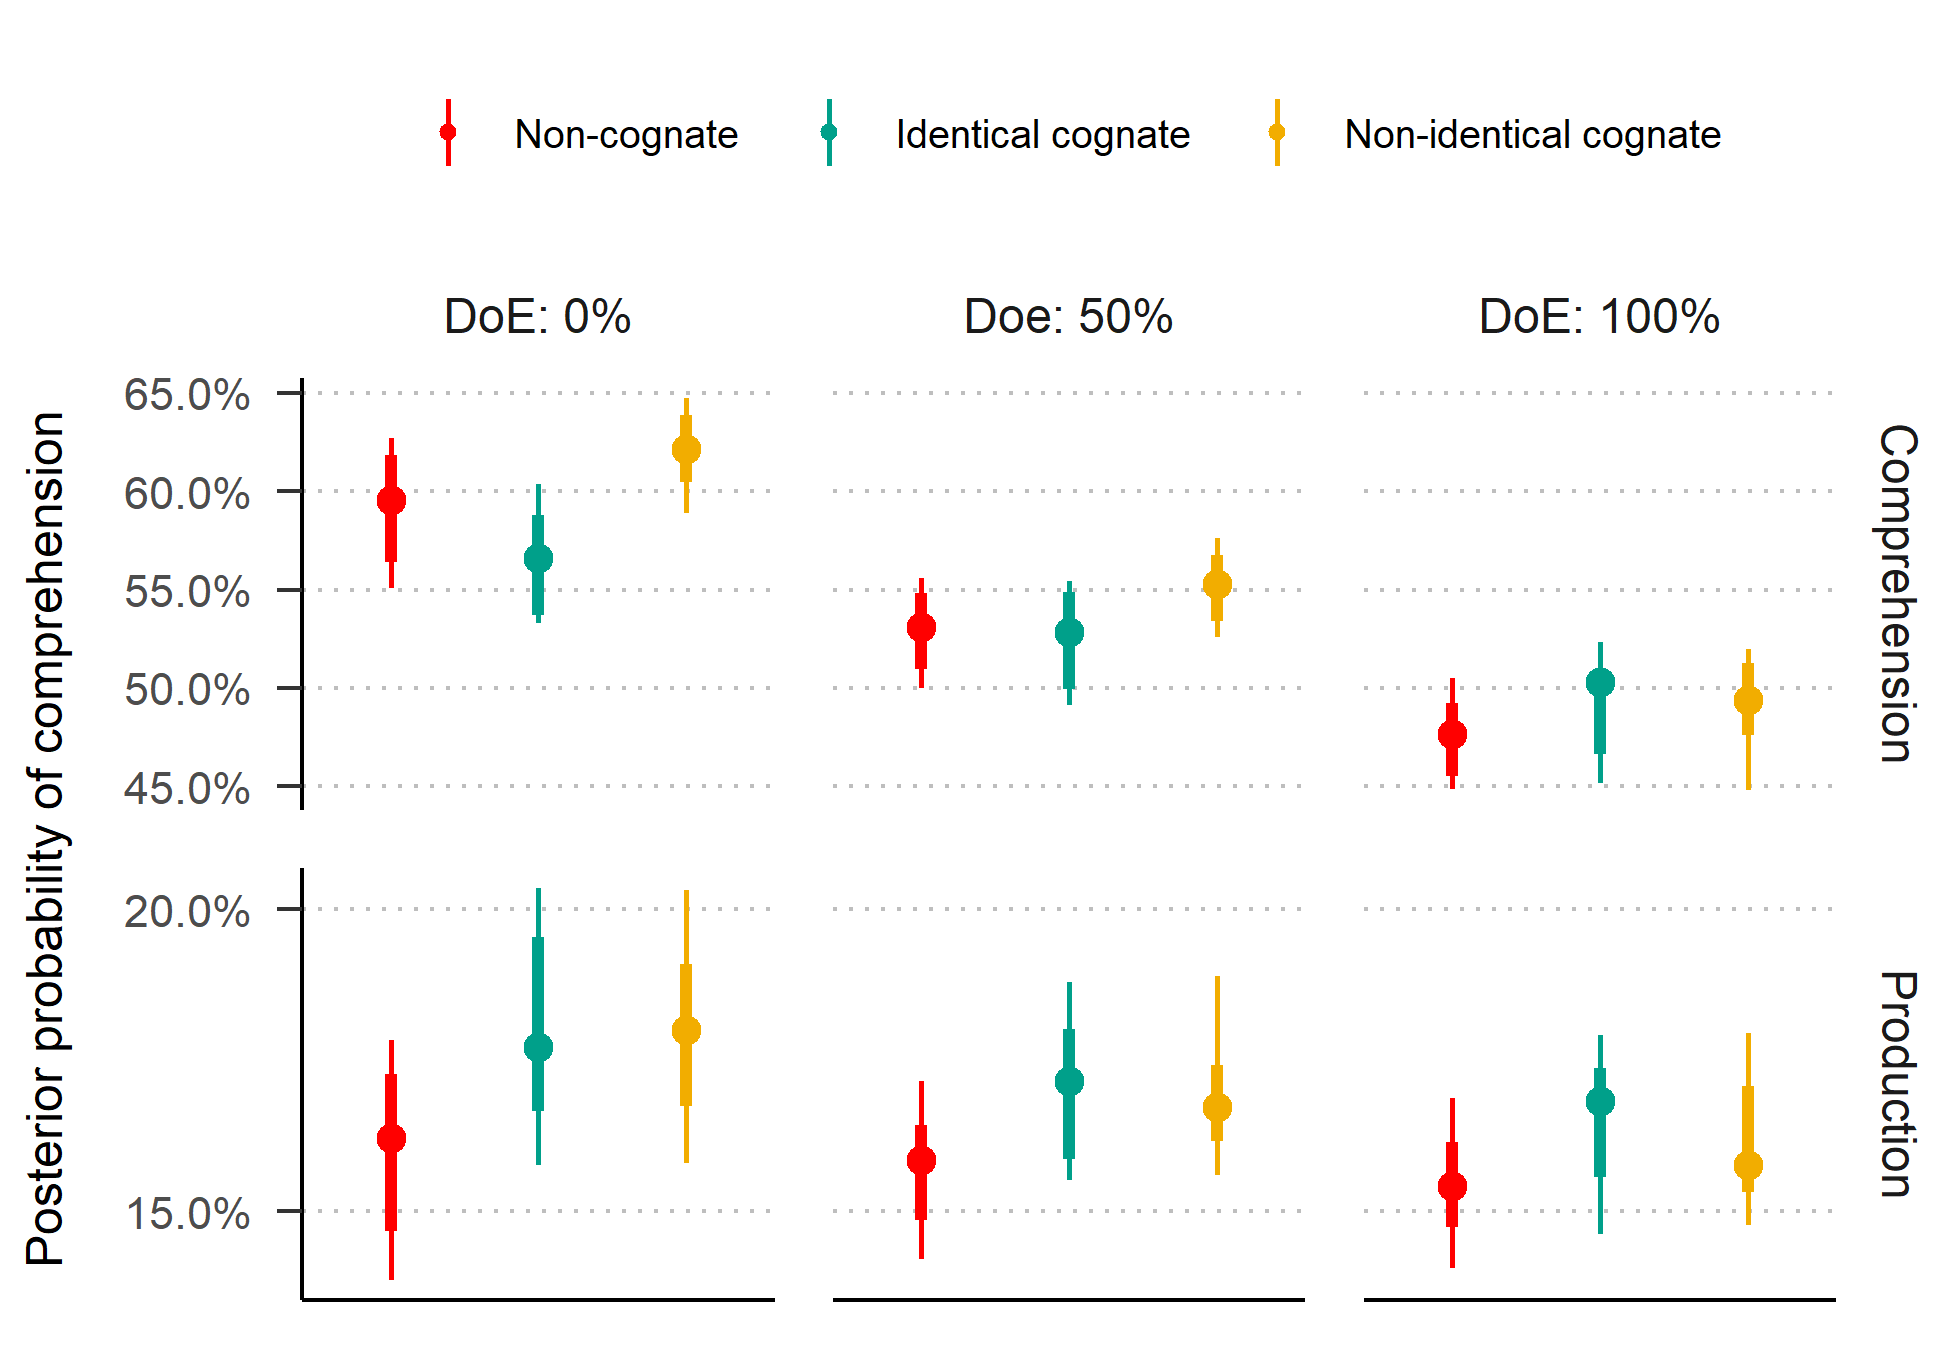
\includegraphics[width=0.8\linewidth]{manuscript_files/figure-latex/emmeans-1}

\}

\textbackslash caption\{Expected marginal mean and 95\% credible interval of the posterior probability of comprehension and production for identical cognates, non-identical cognates, and non cognates, plotted separately for three levels of degree of exposue to the language: 0\% (no exposure, monolingual), 50\% (exposed half of the time, balanced bilingual), and 100\% (exposed all of the time, monolingual). Dots represent the mean, and error bars represent the range of values within the true values is contained with 50\% (thick line) and 95\% (thin line) cprobability, given the data.\}\label{fig:emmeans}
\textbackslash end\{figure\}

\hypertarget{discussion}{%
\section{Discussion}\label{discussion}}

\hypertarget{references}{%
\section{References}\label{references}}

\begingroup
\setlength{\parindent}{-0.5in}
\setlength{\leftskip}{0.5in}

\hypertarget{refs}{}
\begin{CSLReferences}{1}{0}
\leavevmode\vadjust pre{\hypertarget{ref-agresti2003categorical}{}}%
Agresti, A. (2003). \emph{Categorical data analysis} (Vol. 482). John Wiley \& Sons.

\leavevmode\vadjust pre{\hypertarget{ref-arslan2020formr}{}}%
Arslan, R. C., Walther, M. P., \& Tata, C. S. (2020). Formr: A study framework allowing for automated feedback generation and complex longitudinal experience-sampling studies using r. \emph{Behavior Research Methods}, \emph{52}(1), 376--387.

\leavevmode\vadjust pre{\hypertarget{ref-barr2013random}{}}%
Barr, D. J., Levy, R., Scheepers, C., \& Tily, H. J. (2013). Random effects structure for confirmatory hypothesis testing: Keep it maximal. \emph{Journal of Memory and Language}, \emph{68}(3), 255--278.

\leavevmode\vadjust pre{\hypertarget{ref-bergelson2020comprehension}{}}%
Bergelson, E. (2020). The comprehension boost in early word learning: Older infants are better learners. \emph{Child Development Perspectives}, \emph{14}(3), 142--149.

\leavevmode\vadjust pre{\hypertarget{ref-bergelson2012months}{}}%
Bergelson, E., \& Swingley, D. (2012). At 6--9 months, human infants know the meanings of many common nouns. \emph{Proceedings of the National Academy of Sciences}, \emph{109}(9), 3253--3258.

\leavevmode\vadjust pre{\hypertarget{ref-bergelson2015early}{}}%
Bergelson, E., \& Swingley, D. (2015). Early word comprehension in infants: Replication and extension. \emph{Language Learning and Development}, \emph{11}(4), 369--380.

\leavevmode\vadjust pre{\hypertarget{ref-bloom2002children}{}}%
Bloom, P. (2002). \emph{How children learn the meanings of words}. MIT press.

\leavevmode\vadjust pre{\hypertarget{ref-bosch2014first}{}}%
Bosch, L., \& Ramon-Casas, M. (2014). First translation equivalents in bilingual toddlers' expressive vocabulary: {Does} form similarity matter? \emph{International Journal of Behavioral Development}, \emph{38}(4), 317--322. \url{https://doi.org/10.1177/0165025414532559}

\leavevmode\vadjust pre{\hypertarget{ref-braginsky2018childesr}{}}%
Braginsky, M., Sanchez, A., \& Yurovsky, D. (2018). Childesr: Accessing the `CHILDES'database. \emph{R Package Version 0.1. 0}.

\leavevmode\vadjust pre{\hypertarget{ref-braginsky2019consistency}{}}%
Braginsky, Mika, Yurovsky, D., Marchman, V. A., \& Frank, M. C. (2019). Consistency and variability in children's word learning across languages. \emph{Open Mind}, \emph{3}, 52--67.

\leavevmode\vadjust pre{\hypertarget{ref-burkner2017brms}{}}%
Bürkner, P.-C. (2017). Brms: An r package for bayesian multilevel models using stan. \emph{Journal of Statistical Software}, \emph{80}(1), 1--28.

\leavevmode\vadjust pre{\hypertarget{ref-carpenter2017stan}{}}%
Carpenter, B., Gelman, A., Hoffman, M. D., Lee, D., Goodrich, B., Betancourt, M., \ldots{} Riddell, A. (2017). Stan: A probabilistic programming language. \emph{Journal of Statistical Software}, \emph{76}(1), 1--32.

\leavevmode\vadjust pre{\hypertarget{ref-cattani2014much}{}}%
Cattani, A., Abbot-Smith, K., Farag, R., Krott, A., Arreckx, F., Dennis, I., \& Floccia, C. (2014). How much exposure to english is necessary for a bilingual toddler to perform like a monolingual peer in language tests? \emph{International Journal of Language \& Communication Disorders}, \emph{49}(6), 649--671.

\leavevmode\vadjust pre{\hypertarget{ref-costa2000cognate}{}}%
Costa, A., Caramazza, A., \& Sebastian-Galles, N. (2000). The cognate facilitation effect: Implications for models of lexical access. \emph{Journal of Experimental Psychology: Learning, Memory, and Cognition}, \emph{26}(5), 1283.

\leavevmode\vadjust pre{\hypertarget{ref-david2008individual}{}}%
David, A., \& Wei, L. (2008). Individual differences in the lexical development of french--english bilingual children. \emph{International Journal of Bilingual Education and Bilingualism}, \emph{11}(5), 598--618.

\leavevmode\vadjust pre{\hypertarget{ref-fenson1994variability}{}}%
Fenson, L., Dale, P. S., Reznick, J. S., Bates, E., Thal, D. J., Pethick, S. J., \ldots{} Stiles, J. (1994). Variability in early communicative development. \emph{Monographs of the Society for Research in Child Development}, i--185.

\leavevmode\vadjust pre{\hypertarget{ref-fenson2007macarthur}{}}%
Fenson, L., \& others. (2007). \emph{MacArthur-bates communicative development inventories}. Paul H. Brookes Publishing Company Baltimore, MD.

\leavevmode\vadjust pre{\hypertarget{ref-fernald2013ses}{}}%
Fernald, A., Marchman, V. A., \& Weisleder, A. (2013). SES differences in language processing skill and vocabulary are evident at 18 months. \emph{Developmental Science}, \emph{16}(2), 234--248.

\leavevmode\vadjust pre{\hypertarget{ref-floccia2018introduction}{}}%
Floccia, C., Sambrook, T. D., Delle Luche, C., Kwok, R., Goslin, J., White, L., \ldots{} others. (2018). I: INTRODUCTION. \emph{Monographs of the Society for Research in Child Development}, \emph{83}(1), 7--29.

\leavevmode\vadjust pre{\hypertarget{ref-frank2021variability}{}}%
Frank, M. C., Braginsky, M., Yurovsky, D., \& Marchman, V. A. (2021). \emph{Variability and consistency in early language learning: The wordbank project}. MIT Press.

\leavevmode\vadjust pre{\hypertarget{ref-gelman2020regression}{}}%
Gelman, A., Hill, J., \& Vehtari, A. (2020). \emph{Regression and other stories}. Cambridge University Press.

\leavevmode\vadjust pre{\hypertarget{ref-gelman1992inference}{}}%
Gelman, A., \& Rubin, D. B. (1992). Inference from iterative simulation using multiple sequences. \emph{Statistical Science}, \emph{7}(4), 457--472.

\leavevmode\vadjust pre{\hypertarget{ref-goldfield1990early}{}}%
Goldfield, B. A., \& Reznick, J. S. (1990). Early lexical acquisition: Rate, content, and the vocabulary spurt. \emph{Journal of Child Language}, \emph{17}(1), 171--183.

\leavevmode\vadjust pre{\hypertarget{ref-gonzalez2020bilingual}{}}%
Gonzalez-Barrero, A. M., Schott, E., \& Byers-Heinlein, K. (2020). Bilingual adjusted vocabulary: A developmentally-informed bilingual vocabulary measure.

\leavevmode\vadjust pre{\hypertarget{ref-hamilton2000infant}{}}%
Hamilton, A., Plunkett, K., \& Schafer, G. (2000). Infant vocabulary development assessed with a british communicative development inventory. \emph{Journal of Child Language}, \emph{27}(3), 689--705.

\leavevmode\vadjust pre{\hypertarget{ref-hoff2012dual}{}}%
Hoff, E., Core, C., Place, S., Rumiche, R., Señor, M., \& Parra, M. (2012). Dual language exposure and early bilingual development. \emph{Journal of Child Language}, \emph{39}(1), 1.

\leavevmode\vadjust pre{\hypertarget{ref-hoshino2008cognate}{}}%
Hoshino, N., \& Kroll, J. F. (2008). Cognate effects in picture naming: Does cross-language activation survive a change of script? \emph{Cognition}, \emph{106}(1), 501--511.

\leavevmode\vadjust pre{\hypertarget{ref-jones2019children}{}}%
Jones, S., \& Brandt, S. (2019). Do children really acquire dense neighbourhoods? \emph{Journal of Child Language}, \emph{46}(6), 1260--1273.

\leavevmode\vadjust pre{\hypertarget{ref-jusczyk1995infants}{}}%
Jusczyk, P. W., \& Aslin, R. N. (1995). Infants' detection of the sound patterns of words in fluent speech. \emph{Cognitive Psychology}, \emph{29}(1), 1--23.

\leavevmode\vadjust pre{\hypertarget{ref-kachergis2021toward}{}}%
Kachergis, G., Marchman, V. A., \& Frank, M. C. (2021). Toward a {``standard model''} of early language learning.

\leavevmode\vadjust pre{\hypertarget{ref-R-tidybayes}{}}%
Kay, M. (2020). \emph{{tidybayes}: Tidy data and geoms for {Bayesian} models}. \url{https://doi.org/10.5281/zenodo.1308151}

\leavevmode\vadjust pre{\hypertarget{ref-levenshtein1966binary}{}}%
Levenshtein, V. I., \& others. (1966). Binary codes capable of correcting deletions, insertions, and reversals. In \emph{Soviet physics doklady} (Vol. 10, pp. 707--710). Soviet Union.

\leavevmode\vadjust pre{\hypertarget{ref-magnusson2019bayesian}{}}%
Magnusson, M., Andersen, M., Jonasson, J., \& Vehtari, A. (2019). Bayesian leave-one-out cross-validation for large data. In \emph{International conference on machine learning} (pp. 4244--4253). PMLR.

\leavevmode\vadjust pre{\hypertarget{ref-mayor2011statistical}{}}%
Mayor, J., \& Plunkett, K. (2011). A statistical estimate of infant and toddler vocabulary size from CDI analysis. \emph{Developmental Science}, \emph{14}(4), 769--785.

\leavevmode\vadjust pre{\hypertarget{ref-mcelreath2018statistical}{}}%
McElreath, R. (2018). \emph{Statistical rethinking: A bayesian course with examples in r and stan}. Chapman; Hall/CRC.

\leavevmode\vadjust pre{\hypertarget{ref-nelson1973structure}{}}%
Nelson, K. (1973). Structure and strategy in learning to talk. \emph{Monographs of the Society for Research in Child Development}, 1--135.

\leavevmode\vadjust pre{\hypertarget{ref-oller2002language}{}}%
Oller, D. K., \& Eilers, R. E. (2002). \emph{Language and literacy in bilingual children} (Vol. 2). Multilingual Matters.

\leavevmode\vadjust pre{\hypertarget{ref-patterson2004comparing}{}}%
Patterson, J. L. (2004). Comparing bilingual and monolingual toddlers' expressive vocabulary size.

\leavevmode\vadjust pre{\hypertarget{ref-patterson2004bilingual}{}}%
Patterson, J., Pearson, B., \& Goldstein, B. (2004). Bilingual language development and disorders in spanish--english speakers.

\leavevmode\vadjust pre{\hypertarget{ref-pearson1994patterns}{}}%
Pearson, B. Z., \& Fernández, S. C. (1994). Patterns of interaction in the lexical growth in two languages of bilingual infants and toddlers. \emph{Language Learning}, \emph{44}(4), 617--653.

\leavevmode\vadjust pre{\hypertarget{ref-pearson1993lexical}{}}%
Pearson, B. Z., Fernández, S. C., \& Oller, D. K. (1993). Lexical development in bilingual infants and toddlers: Comparison to monolingual norms. \emph{Language Learning}, \emph{43}(1), 93--120.

\leavevmode\vadjust pre{\hypertarget{ref-petitto2001bilingual}{}}%
Petitto, L. A., Katerelos, M., Levy, B. G., Gauna, K., Tétreault, K., \& Ferraro, V. (2001). Bilingual signed and spoken language acquisition from birth: Implications for the mechanisms underlying early bilingual language acquisition. \emph{Journal of Child Language}, \emph{28}(2), 453--496.

\leavevmode\vadjust pre{\hypertarget{ref-poulin2013lexical}{}}%
Poulin-Dubois, D., Bialystok, E., Blaye, A., Polonia, A., \& Yott, J. (2013). Lexical access and vocabulary development in very young bilinguals. \emph{International Journal of Bilingualism}, \emph{17}(1), 57--70.

\leavevmode\vadjust pre{\hypertarget{ref-R-base}{}}%
R Core Team. (2020). \emph{R: A language and environment for statistical computing}. Vienna, Austria: R Foundation for Statistical Computing. Retrieved from \url{https://www.R-project.org/}

\leavevmode\vadjust pre{\hypertarget{ref-schad2020capitalize}{}}%
Schad, D. J., Vasishth, S., Hohenstein, S., \& Kliegl, R. (2020). How to capitalize on a priori contrasts in linear (mixed) models: A tutorial. \emph{Journal of Memory and Language}, \emph{110}, 104038.

\leavevmode\vadjust pre{\hypertarget{ref-schelletter2002effect}{}}%
Schelletter, C. (2002). The effect of form similarity on bilingual children's lexical development. \emph{Bilingualism: Language and Cognition}, \emph{5}(2), 93--107. \url{https://doi.org/10.1017/S1366728902000214}

\leavevmode\vadjust pre{\hypertarget{ref-smithson2014bilingualism}{}}%
Smithson, L., Paradis, J., \& Nicoladis, E. (2014). Bilingualism and receptive vocabulary achievement: Could sociocultural context make a difference? \emph{Bilingualism: Language and Cognition}, \emph{17}(4), 810--821.

\leavevmode\vadjust pre{\hypertarget{ref-tardif2008baby}{}}%
Tardif, T., Fletcher, P., Liang, W., Zhang, Z., Kaciroti, N., \& Marchman, V. A. (2008). Baby's first 10 words. \emph{Developmental Psychology}, \emph{44}(4), 929.

\leavevmode\vadjust pre{\hypertarget{ref-thierry2007brain}{}}%
Thierry, G., \& Wu, Y. J. (2007). Brain potentials reveal unconscious translation during foreign-language comprehension. \emph{Proceedings of the National Academy of Sciences}, \emph{104}(30), 12530--12535.

\leavevmode\vadjust pre{\hypertarget{ref-thordardottir2006bilingual}{}}%
Thordardottir, E., Rothenberg, A., Rivard, M.-E., \& Naves, R. (2006). Bilingual assessment: Can overall proficiency be estimated from separate measurement of two languages? \emph{Journal of Multilingual Communication Disorders}, \emph{4}(1), 1--21.

\leavevmode\vadjust pre{\hypertarget{ref-tincoff1999some}{}}%
Tincoff, R., \& Jusczyk, P. W. (1999). Some beginnings of word comprehension in 6-month-olds. \emph{Psychological Science}, \emph{10}(2), 172--175.

\leavevmode\vadjust pre{\hypertarget{ref-van2014subtlex}{}}%
Van Heuven, W. J., Mandera, P., Keuleers, E., \& Brysbaert, M. (2014). SUBTLEX-UK: A new and improved word frequency database for british english. \emph{Quarterly Journal of Experimental Psychology}, \emph{67}(6), 1176--1190.

\leavevmode\vadjust pre{\hypertarget{ref-vehtari2017practical}{}}%
Vehtari, A., Gelman, A., \& Gabry, J. (2017). Practical bayesian model evaluation using leave-one-out cross-validation and WAIC. \emph{Statistics and Computing}, \emph{27}(5), 1413--1432.

\leavevmode\vadjust pre{\hypertarget{ref-von2012language}{}}%
Von Holzen, K., \& Mani, N. (2012). Language nonselective lexical access in bilingual toddlers. \emph{Journal of Experimental Child Psychology}, \emph{113}(4), 569--586.

\leavevmode\vadjust pre{\hypertarget{ref-R-tidyverse}{}}%
Wickham, H., Averick, M., Bryan, J., Chang, W., McGowan, L. D., François, R., \ldots{} Yutani, H. (2019). Welcome to the {tidyverse}. \emph{Journal of Open Source Software}, \emph{4}(43), 1686. \url{https://doi.org/10.21105/joss.01686}

\leavevmode\vadjust pre{\hypertarget{ref-zipf1949human}{}}%
Zipf, G. K. (1949). Human behavior and the principle of least effort: An introd. To human ecology.

\end{CSLReferences}

\endgroup


\end{document}
